

\documentclass[14pt]{scrartcl} % Font size

%%%%%%%%%%%%%%%%%%%%%%%%%%%%%%%%%%%%%%%%%
% Wenneker Assignment
% Structure Specification File
% Version 2.0 (12/1/2019)
%
% This template originates from:
% http://www.LaTeXTemplates.com
%
% Authors:
% Vel (vel@LaTeXTemplates.com)
% Frits Wenneker
%
% License:
% CC BY-NC-SA 3.0 (http://creativecommons.org/licenses/by-nc-sa/3.0/)
% 
%%%%%%%%%%%%%%%%%%%%%%%%%%%%%%%%%%%%%%%%%

%----------------------------------------------------------------------------------------
%	PACKAGES AND OTHER DOCUMENT CONFIGURATIONS
%----------------------------------------------------------------------------------------

\usepackage{amsmath, amsfonts, amsthm} % Math packages

\usepackage{listings} % Code listings, with syntax highlighting

\usepackage[english]{babel} % English language hyphenation

\usepackage{graphicx} % Required for inserting images
\graphicspath{{Figures/}{./}} % Specifies where to look for included images (trailing slash required)

\usepackage{booktabs} % Required for better horizontal rules in tables

\numberwithin{equation}{section} % Number equations within sections (i.e. 1.1, 1.2, 2.1, 2.2 instead of 1, 2, 3, 4)
\numberwithin{figure}{section} % Number figures within sections (i.e. 1.1, 1.2, 2.1, 2.2 instead of 1, 2, 3, 4)
\numberwithin{table}{section} % Number tables within sections (i.e. 1.1, 1.2, 2.1, 2.2 instead of 1, 2, 3, 4)

\setlength\parindent{0pt} % Removes all indentation from paragraphs

\usepackage{enumitem} % Required for list customisation
\usepackage{caption}
\usepackage{subcaption}
\setlist{noitemsep} % No spacing between list items

%----------------------------------------------------------------------------------------
%	DOCUMENT MARGINS
%----------------------------------------------------------------------------------------

\usepackage{geometry} % Required for adjusting page dimensions and margins

\geometry{
	paper=a4paper, % Paper size, change to letterpaper for US letter size
	top=2.5cm, % Top margin
	bottom=3cm, % Bottom margin
	left=3cm, % Left margin
	right=3cm, % Right margin
	headheight=0.75cm, % Header height
	footskip=1.5cm, % Space from the bottom margin to the baseline of the footer
	headsep=0.75cm, % Space from the top margin to the baseline of the header
	%showframe, % Uncomment to show how the type block is set on the page
}

%----------------------------------------------------------------------------------------
%	FONTS
%----------------------------------------------------------------------------------------

\usepackage[utf8]{inputenc} % Required for inputting international characters
\usepackage[T1]{fontenc} % Use 8-bit encoding

\usepackage{fourier} % Use the Adobe Utopia font for the document

%----------------------------------------------------------------------------------------
%	SECTION TITLES
%----------------------------------------------------------------------------------------

\usepackage{sectsty} % Allows customising section commands

\sectionfont{\vspace{6pt}\centering\normalfont\scshape} % \section{} styling
\subsectionfont{\normalfont\bfseries} % \subsection{} styling
\subsubsectionfont{\normalfont\itshape} % \subsubsection{} styling
\paragraphfont{\normalfont\scshape} % \paragraph{} styling

%----------------------------------------------------------------------------------------
%	HEADERS AND FOOTERS
%----------------------------------------------------------------------------------------

\usepackage{scrlayer-scrpage} % Required for customising headers and footers

\ohead*{} % Right header
\ihead*{} % Left header
\chead*{} % Centre header

\ofoot*{} % Right footer
\ifoot*{} % Left footer
\cfoot*{\pagemark} % Centre footer


\usepackage{xcolor}
\usepackage{multirow}
\usepackage{multicol}
\usepackage{colortbl}

\usepackage{algpseudocode} % Include the file specifying the document structure and custom commands

%----------------------------------------------------------------------------------------
%	TITLE SECTION
%----------------------------------------------------------------------------------------

\title{	
	\normalfont\normalsize
	\textsc{Department of Computer Science and Engineering, BUET}\\ % Your university, school and/or department name(s)
	\vspace{25pt} % Whitespace
	\rule{\linewidth}{0.5pt}\\ % Thin top horizontal rule
	\vspace{20pt} % Whitespace
	{\huge NS2 Project Report}\\ % The assignment title
	\vspace{12pt} % Whitespace
	\rule{\linewidth}{2pt}\\ % Thick bottom horizontal rule
	\vspace{12pt} % Whitespace
}

\author{\LARGE Ruhul Azgor \\ 1805091} % Your name

\date{\normalsize\today} % Today's date (\today) or a custom date

\begin{document}

\maketitle % Print the title

%----------------------------------------------------------------------------------------
%	FIGURE EXAMPLE
%----------------------------------------------------------------------------------------

\section*{}

\begin{figure}[h] % [h] forces the figure to be output where it is defined in the code (it suppresses floating)
	\centering
	
\includegraphics[width=0.5\columnwidth]{Figures/BUET_LOGO.svg.png} % Example image
	 
\end{figure}

%------------------------------------------------
\pagebreak
%\paragraph{My student ID is %1805091.$91\%8=3$. So, I have simulated %Wireless 802.15.4 (static) ( section-1) and %Wireless 802.11 (mobile) (section-2) %network.In the section-3, I have simulated %modified AODV routing protocol in Wireless %802.11 (mobile) network. }

%\section{Wireless 802.15.4 (static)}
\subsection{Description of the simulation}
The simulation is based on the IEEE 802.15.4(static) standard. Routing is based on the dsdv protocol. The simulation is based on the ns-2 simulator. The simulation is based on the following parameters:
\begin{itemize}
    \item Channel: Wireless channel
    \item Propagation: Two-ray ground
    \item Antenna: Omnidirectional
    \item Link: 802.15.4
    \item Queue: Drop-tail
    \item Routing: DSDV
    \item Mobility: Static
    \item Position: Grid
    \item Area: 2*(tx\_range)m x 2*(tx\_range)m
    \item Flow: Random source to random destination
    \item Packet size: 64 bytes
    \item Number of nodes: Variable
    \item Number of flows: Variable
    \item Packet rate: Variable
    \item Tx Coverage: Variable
    \item Simulation time: 60 seconds
\end{itemize}

\subsection{Results}
\subsubsection{Varying Number of Nodes}
Baseline parameters are as follows:
\begin{itemize}
    \item Number of flows: 20
    \item Packet rate: 100 packets per second
    \item Tx Coverage: 300m
\end{itemize}
The number of nodes is varied from 20 to 100 in steps of 20.
See Figure \ref{node_throughput} ,\ref{node_delay} , \ref{node_delivery} , \ref{node_drop}, \ref{node_energy} , \ref{node_energy_per_byte} and \ref{node_per_node_throughput} for the result.
\begin{figure}[h]
\begin{subfigure}{.5\textwidth}
  \centering
  % include first image
  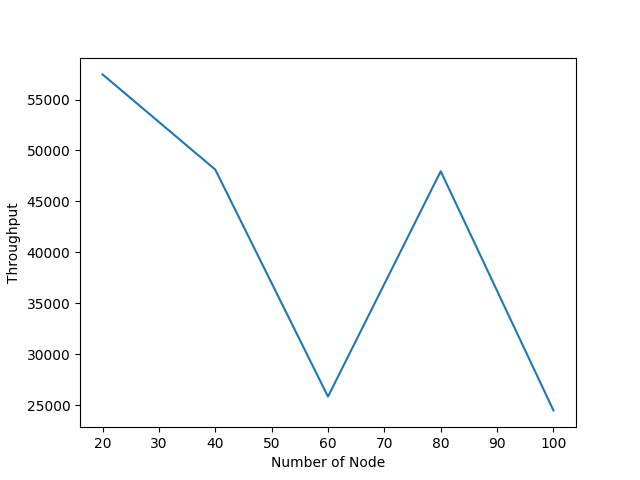
\includegraphics[width=.8\linewidth]{_15_4_static/NumberofNodevsThroughput.png}
     \caption{Number of Nodes Vs Throughput}
    \label{node_throughput}
\end{subfigure}
\begin{subfigure}{.5\textwidth}
  \centering
  % include second image
  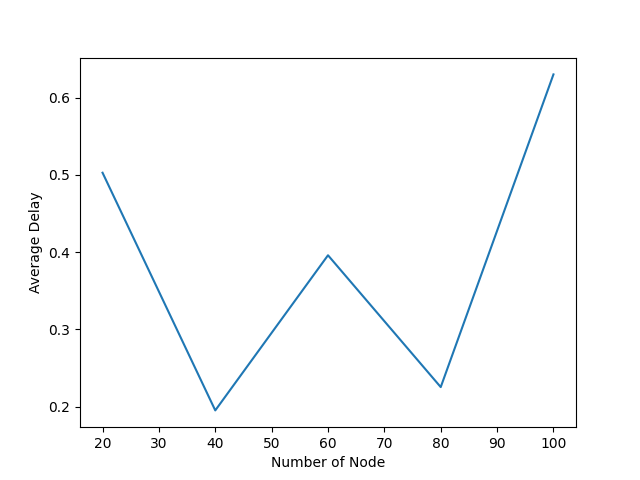
\includegraphics[width=.8\linewidth]{_15_4_static/NumberofNodevsAverageDelay.png}
    \caption{Number of Nodes Vs Average Delay}
     \label{node_delay}
\end{subfigure}
\begin{subfigure}{.5\textwidth}
  \centering
  % include third image
  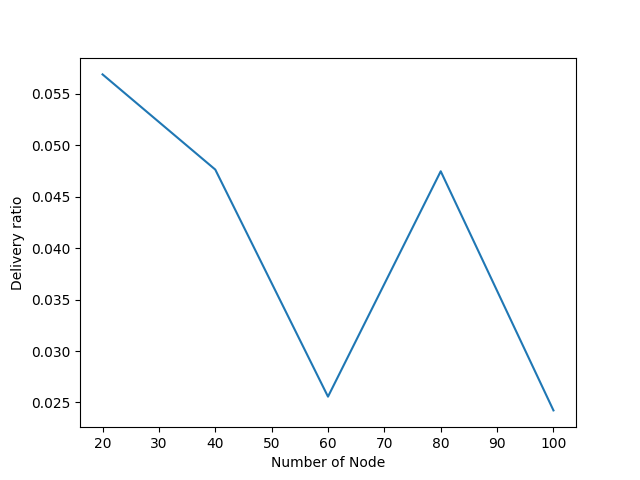
\includegraphics[width=.8\linewidth]{_15_4_static/NumberofNodevsDeliveryRatio.png}
     \caption{Number of Nodes Vs Delivary Ratio}
     \label{node_delivery}
\end{subfigure}
\begin{subfigure}{.5\textwidth}
  \centering
  % include fourth image
  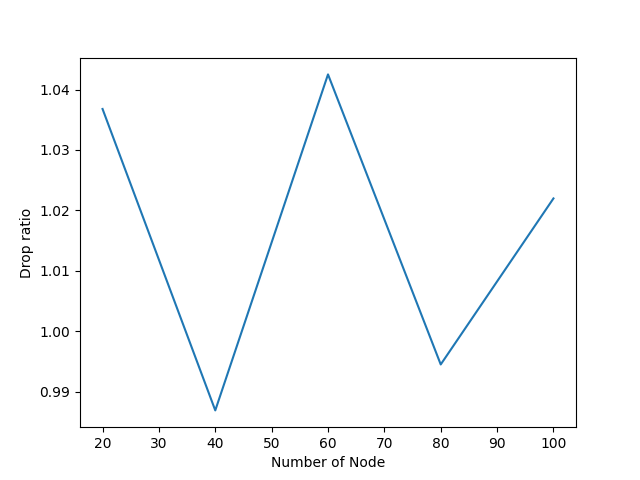
\includegraphics[width=.8\linewidth]{_15_4_static/NumberofNodevsDropRatio.png}
     \caption{Number of Nodes Vs Drop Ratio}
     \label{node_drop}
\end{subfigure}
\begin{subfigure}{.5\textwidth}
  \centering
  % include fifth image
  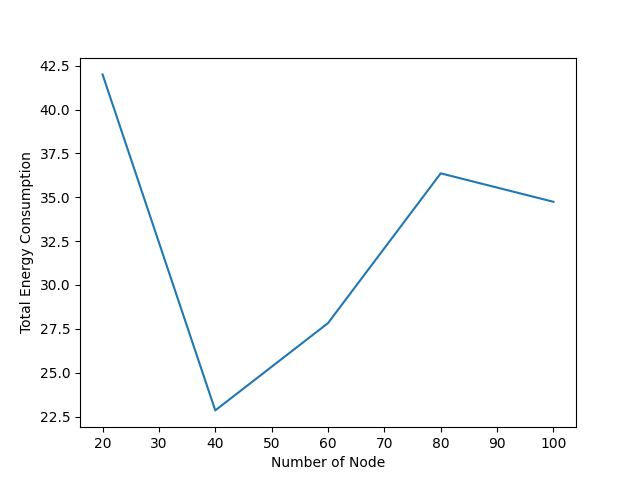
\includegraphics[width=.8\linewidth]{_15_4_static/NumberofNodevsTotalEnergyConsumption.png}
     \caption{Number of Nodes Vs Energy Consumption}
     \label{node_energy}
\end{subfigure}
\begin{subfigure}{.5\textwidth}
  \centering
  % include sixth image
  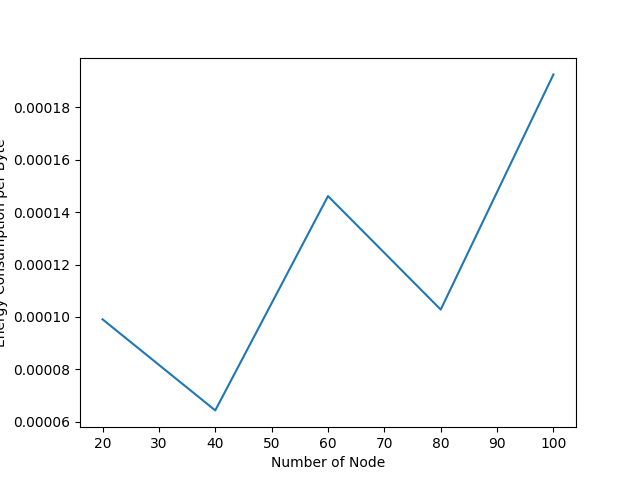
\includegraphics[width=.8\linewidth]{_15_4_static/NumberofNodevsEnergyConsumptionperByte.png}
     \caption{Number of Nodes Vs Energy Per Byte}
     \label{node_energy_per_byte}
\end{subfigure}
\caption{Varying Number of Nodes}
\label{fig:varyingNode}
\end{figure}
\begin{figure}[h]
\begin{subfigure}{.5\textwidth}
  \centering
  % include first image
  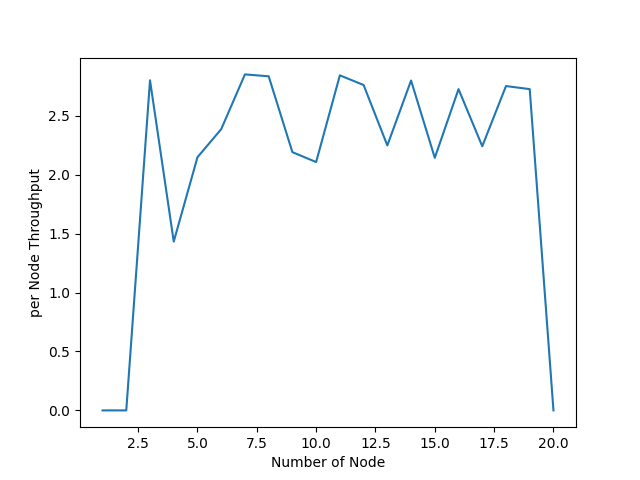
\includegraphics[width=.8\linewidth]{_15_4_static/NumberofNode(20)vsperNodeThroughput.png}
     \caption{Number of Nodes(20) Vs Throughput per Node}
 \end{subfigure}
\begin{subfigure}{.5\textwidth}
  \centering
  % include second image
  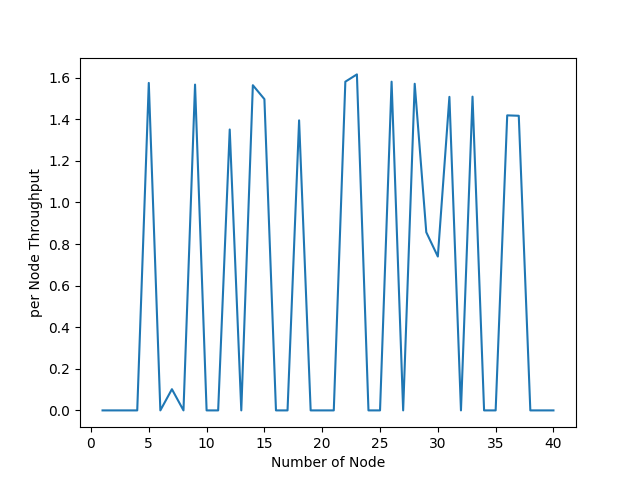
\includegraphics[width=.8\linewidth]{_15_4_static/NumberofNode(40)vsperNodeThroughput.png}
     \caption{Number of Nodes(40) Vs Throughput per Node}
    \end{subfigure}
\begin{subfigure}{.5\textwidth}
    \centering
    % include third image
    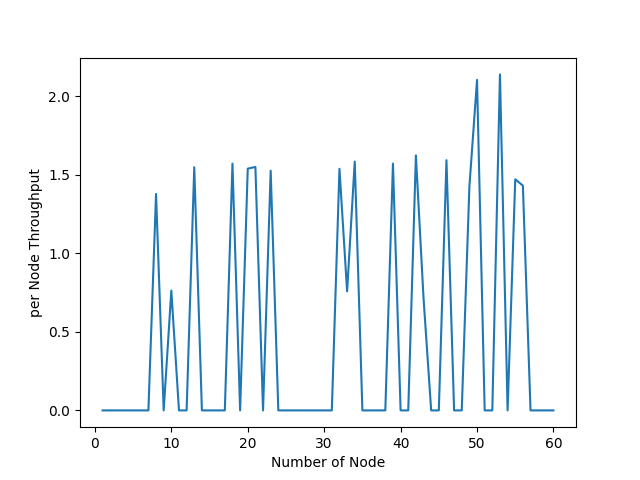
\includegraphics[width=.8\linewidth]{_15_4_static/NumberofNode(60)vsperNodeThroughput.png}
         \caption{Number of Nodes(60) Vs Throughput per Node}
        \end{subfigure}
\begin{subfigure}{.5\textwidth}
    \centering
    % include fourth image
    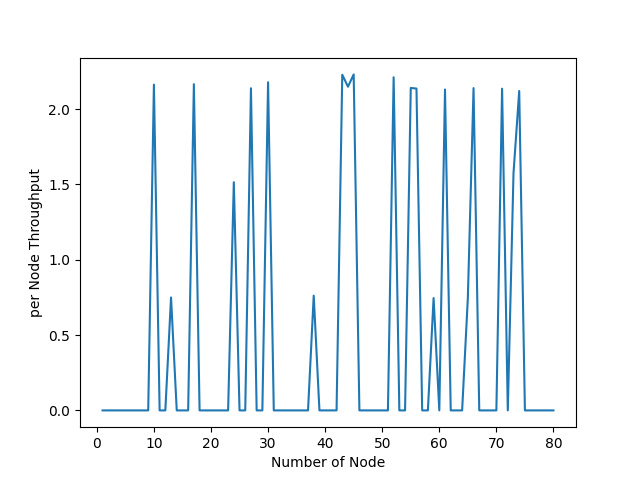
\includegraphics[width=.8\linewidth]{_15_4_static/NumberofNode(80)vsperNodeThroughput.png}
         \caption{Number of Nodes(80) Vs Throughput per Node}
        \end{subfigure}
\begin{subfigure}{.5\textwidth}
    \centering
    % include fifth image
    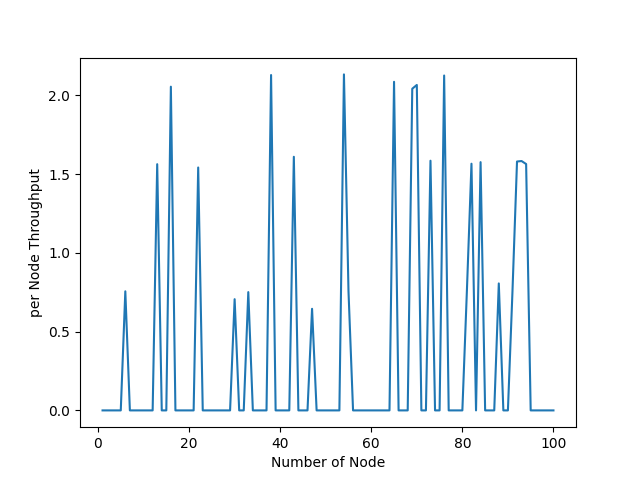
\includegraphics[width=.8\linewidth]{_15_4_static/NumberofNode(100)vsperNodeThroughput.png}
         \caption{Number of Nodes(100) Vs Throughput per Node}
        \end{subfigure}
\caption{Varying Number of Nodes (Throughput per Node)}
\label{node_per_node_throughput}
\end{figure}

\subsubsection{Varying Number of Flows}
Baseline parameters are as follows:
\begin{itemize}
    \item Number of nodes: 40
    \item Packet rate: 100 packets per second
    \item Tx Coverage: 300m
\end{itemize}
The number of flows is varied from 10 to 50 in steps of 10.
See Figure \ref{flow_throughput} ,\ref{flow_delay} , \ref{flow_delivery} , \ref{flow_drop}, \ref{flow_energy} , \ref{flow_energy_per_byte} and \ref{flow_per_node_throughput} for the result.
\begin{figure}[h]
\begin{subfigure}{.5\textwidth}
  \centering
  % include first image
  \includegraphics[width=.8\linewidth]{_15_4_static/NumberofFlowvsThroughput.png}
     \caption{Number of Flows Vs Throughput}
    \label{flow_throughput}
\end{subfigure}
\begin{subfigure}{.5\textwidth}
  \centering
  % include second image
  \includegraphics[width=.8\linewidth]{_15_4_static/NumberofFlowvsAverageDelay.png}
    \caption{Number of Flows Vs Average Delay}
     \label{flow_delay}
\end{subfigure}
\begin{subfigure}{.5\textwidth}
  \centering
  % include third image
  \includegraphics[width=.8\linewidth]{_15_4_static/NumberofFlowvsDeliveryRatio.png}
     \caption{Number of Flows Vs Delivary Ratio}
     \label{flow_delivery}
\end{subfigure}
\begin{subfigure}{.5\textwidth}
  \centering
  % include fourth image
  \includegraphics[width=.8\linewidth]{_15_4_static/NumberofFlowvsDropRatio.png}
     \caption{Number of Flows Vs Drop Ratio}
     \label{flow_drop}
\end{subfigure}
\begin{subfigure}{.5\textwidth}
  \centering
  % include fifth image
  \includegraphics[width=.8\linewidth]{_15_4_static/NumberofFlowvsTotalEnergyConsumption.png}
     \caption{Number of Flows Vs Energy Consumption}
     \label{flow_energy}
\end{subfigure}
\begin{subfigure}{.5\textwidth}
  \centering
  % include sixth image
  \includegraphics[width=.8\linewidth]{_15_4_static/NumberofFlowvsEnergyConsumptionperByte.png}
     \caption{Number of Flows Vs Energy Per Byte}
     \label{flow_energy_per_byte}
\end{subfigure}
\caption{Varying Number of Flows}
\label{fig:varyingFlow}
\end{figure}
\begin{figure}[h]
\begin{subfigure}{.5\textwidth}
  \centering
  % include first image
  \includegraphics[width=.8\linewidth]{_15_4_static/NumberofFlow(10)vsperNodeThroughput.png}
     \caption{Number of Flows(10) Vs Throughput per Node}
 \end{subfigure}
\begin{subfigure}{.5\textwidth}
  \centering
  % include second image
  \includegraphics[width=.8\linewidth]{_15_4_static/NumberofFlow(20)vsperNodeThroughput.png}
     \caption{Number of Flows(20) Vs Throughput per Node}
    \end{subfigure}
\begin{subfigure}{.5\textwidth}
    \centering
    % include third image
    \includegraphics[width=.8\linewidth]{_15_4_static/NumberofFlow(30)vsperNodeThroughput.png}
         \caption{Number of Flows(30) Vs Throughput per Node}
        \end{subfigure}
\begin{subfigure}{.5\textwidth}
    \centering
    % include fourth image
    \includegraphics[width=.8\linewidth]{_15_4_static/NumberofFlow(40)vsperNodeThroughput.png}
         \caption{Number of Flows(40) Vs Throughput per Node}
        \end{subfigure}
\begin{subfigure}{.5\textwidth}
    \centering
    % include fifth image
    \includegraphics[width=.8\linewidth]{_15_4_static/NumberofFlow(50)vsperNodeThroughput.png}
         \caption{Number of Flows(50) Vs Throughput per Node}
        \end{subfigure}
\caption{Varying Number of Flows (Throughput per Node)}
\label{flow_per_node_throughput}
\end{figure}

\subsubsection{Varying Packet per Second}
Baseline parameters are as follows:
\begin{itemize}
    \item Number of nodes: 40
    \item Number of flows: 10
    \item Tx Coverage: 300m
\end{itemize}
The packet rate is varied from 100 to 500 packets per second in steps of 100.
See Figure \ref{packet_rate_throughput} ,\ref{packet_rate_delay} , \ref{packet_rate_delivery} , \ref{packet_rate_drop}, \ref{packet_rate_energy} , \ref{packet_rate_energy_per_byte} and \ref{packet_rate_per_node_throughput} for the result.
\begin{figure}[h]
\begin{subfigure}{.5\textwidth}
  \centering
  % include first image
  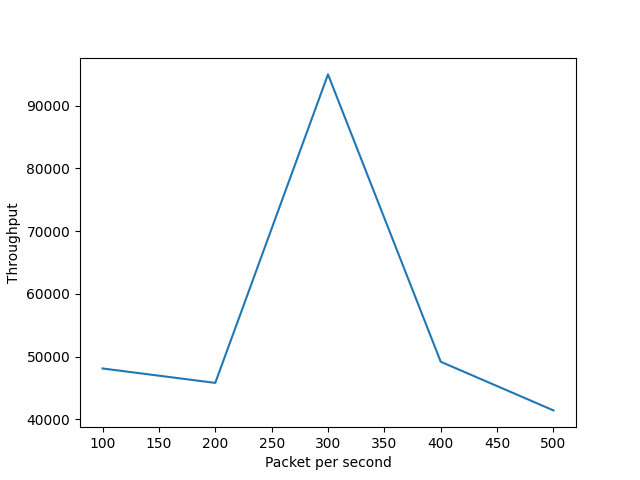
\includegraphics[width=.8\linewidth]{_15_4_static/PacketpersecondvsThroughput.png}
     \caption{Packet Rate Vs Throughput}
    \label{packet_rate_throughput}
\end{subfigure}
\begin{subfigure}{.5\textwidth}
  \centering
  % include second image
  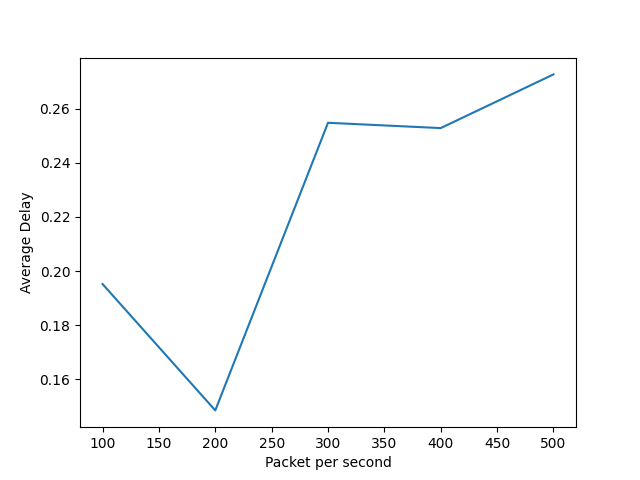
\includegraphics[width=.8\linewidth]{_15_4_static/PacketpersecondvsAverageDelay.png}
    \caption{Packet Rate Vs Average Delay}
     \label{packet_rate_delay}
\end{subfigure}
\begin{subfigure}{.5\textwidth}
  \centering
  % include third image
  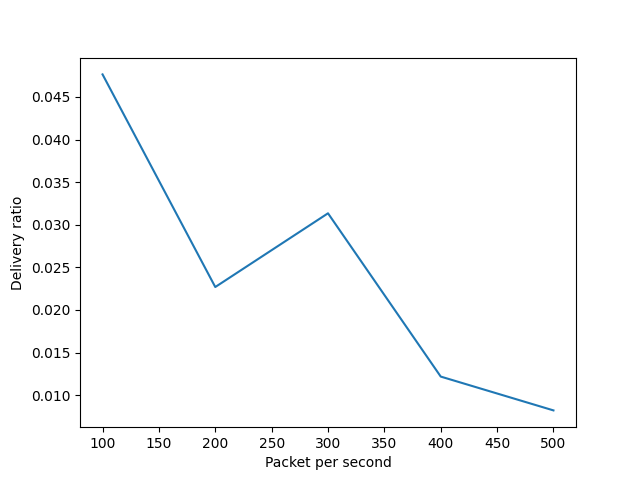
\includegraphics[width=.8\linewidth]{_15_4_static/PacketpersecondvsDeliveryRatio.png}
     \caption{Packet Rate Vs Delivary Ratio}
     \label{packet_rate_delivery}
\end{subfigure}
\begin{subfigure}{.5\textwidth}
  \centering
  % include fourth image
  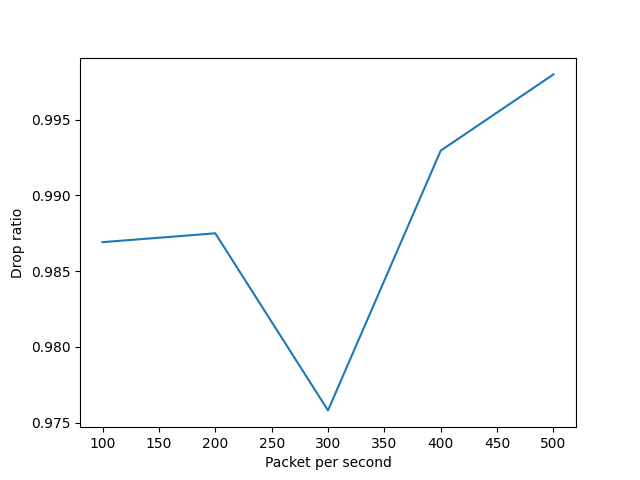
\includegraphics[width=.8\linewidth]{_15_4_static/PacketpersecondvsDropRatio.png}
     \caption{Packet Rate Vs Drop Ratio}
     \label{packet_rate_drop}
\end{subfigure}
\begin{subfigure}{.5\textwidth}
  \centering
  % include fifth image
  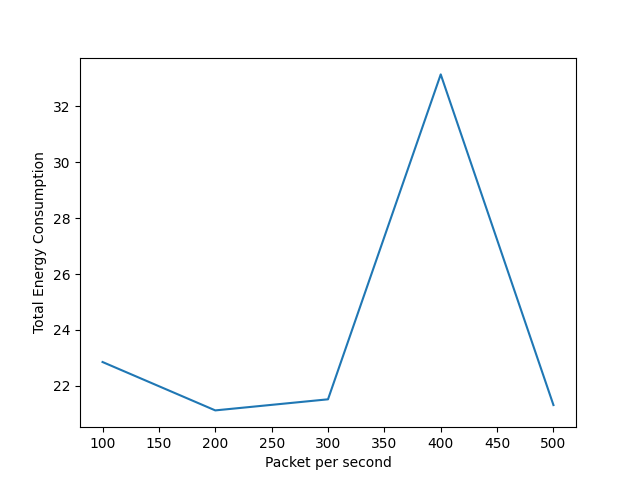
\includegraphics[width=.8\linewidth]{_15_4_static/PacketpersecondvsTotalEnergyConsumption.png}
     \caption{Packet Rate Vs Energy Consumption}
     \label{packet_rate_energy}
\end{subfigure}
\begin{subfigure}{.5\textwidth}
  \centering
  % include sixth image
  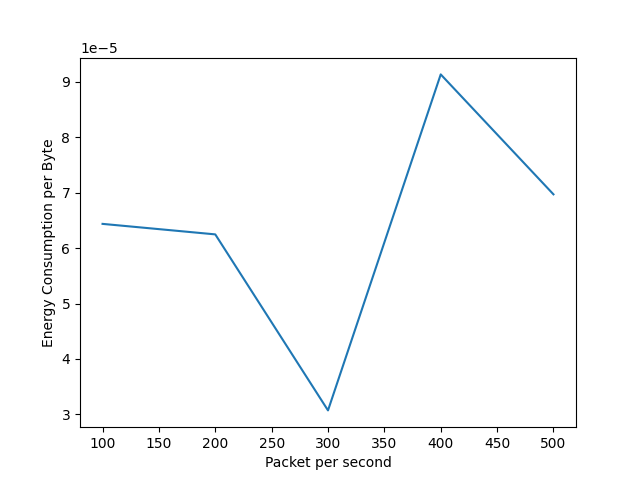
\includegraphics[width=.8\linewidth]{_15_4_static/PacketpersecondvsEnergyConsumptionperByte.png}
     \caption{Packet Rate Vs Energy Per Byte}
     \label{packet_rate_energy_per_byte}
\end{subfigure}
\caption{Varying Packet Rate}
\label{fig:varyingPacketRate}
\end{figure}
\begin{figure}[h]
\begin{subfigure}{.5\textwidth}
  \centering
  % include first image
  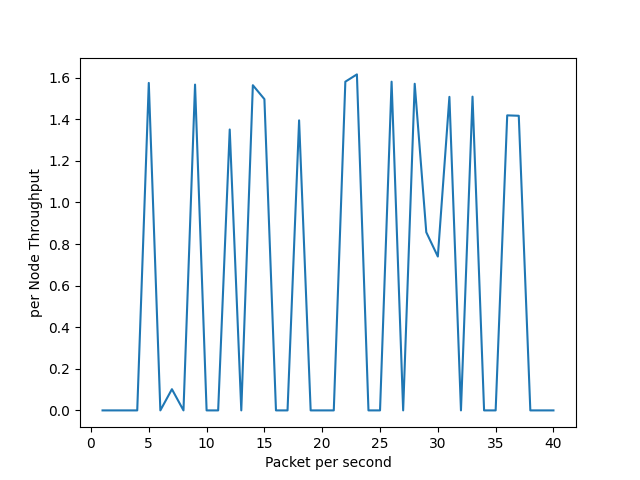
\includegraphics[width=.8\linewidth]{_15_4_static/Packetpersecond(100)vsperNodeThroughput.png}
     \caption{Packet Rate(100) Vs Throughput per Node}
 \end{subfigure}
\begin{subfigure}{.5\textwidth}
  \centering
  % include second image
  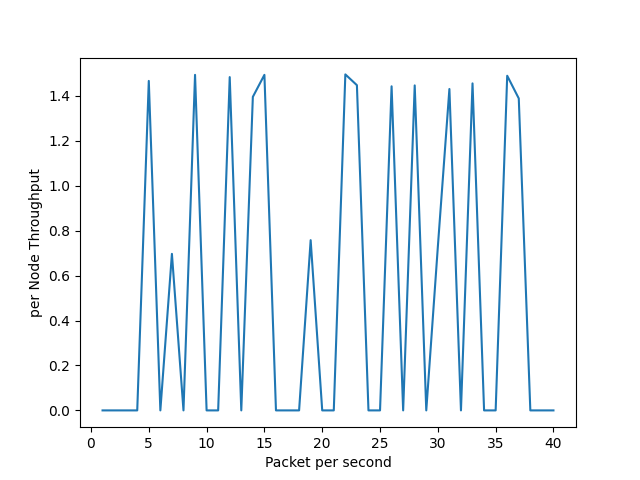
\includegraphics[width=.8\linewidth]{_15_4_static/Packetpersecond(200)vsperNodeThroughput.png}
     \caption{Packet Rate(200) Vs Throughput per Node}
    \end{subfigure}
\begin{subfigure}{.5\textwidth}
    \centering
    % include third image
    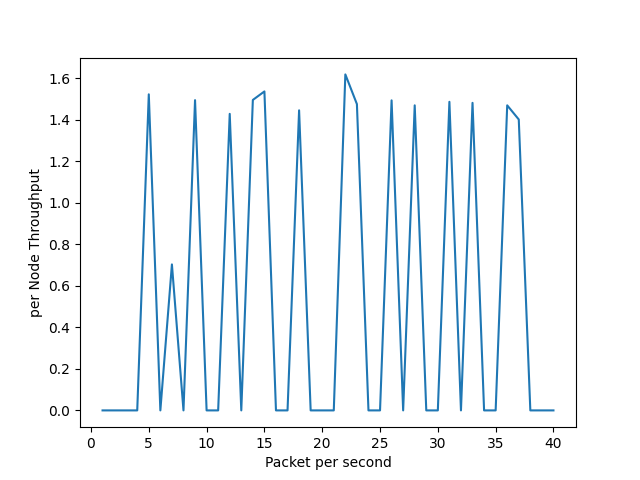
\includegraphics[width=.8\linewidth]{_15_4_static/Packetpersecond(300)vsperNodeThroughput.png}
         \caption{Packet Rate(300) Vs Throughput per Node}
        \end{subfigure}
\begin{subfigure}{.5\textwidth}
    \centering
    % include fourth image
    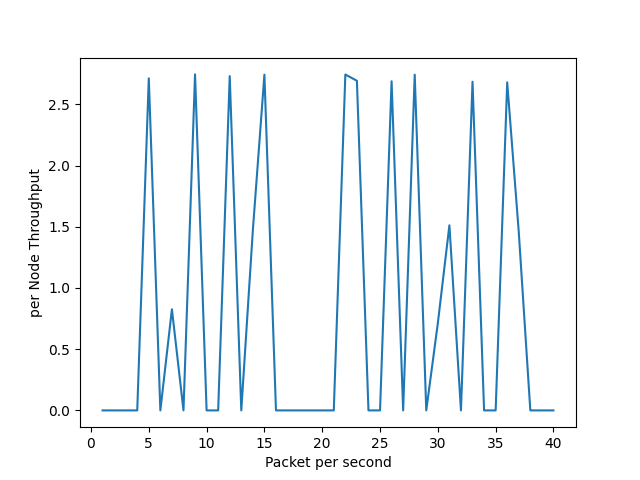
\includegraphics[width=.8\linewidth]{_15_4_static/Packetpersecond(400)vsperNodeThroughput.png}
         \caption{Packet Rate(400) Vs Throughput per Node}
        \end{subfigure}
\begin{subfigure}{.5\textwidth}
    \centering
    % include fifth image
    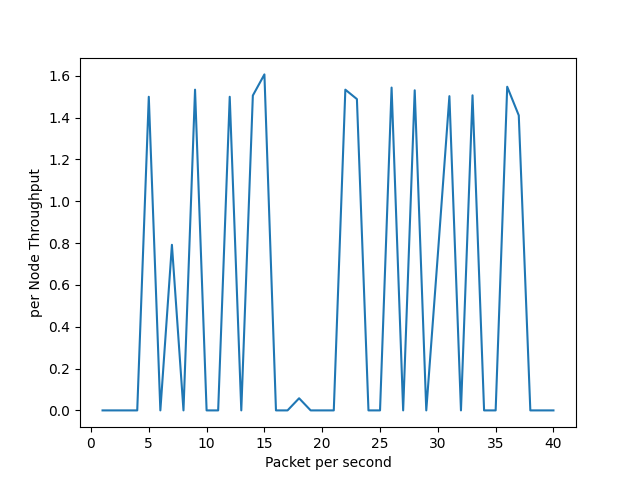
\includegraphics[width=.8\linewidth]{_15_4_static/Packetpersecond(500)vsperNodeThroughput.png}
         \caption{Packet Rate(500) Vs Throughput per Node}
        \end{subfigure}
\caption{Varying Packet Rate (Throughput per Node)}
\label{packet_rate_per_node_throughput}
\end{figure}
\subsubsection{Varying Transmission Range}
Baseline parameters are as follows:
\begin{itemize}
    \item Number of nodes: 40
    \item Number of flows: 10
    \item Packet Rate: 100 packets per second
\end{itemize}
The transmission range is varied from 100 to 500 meters in steps of 100.
See Figure \ref{tx_range_throughput} ,\ref{tx_range_delay} , \ref{tx_range_delivery} , \ref{tx_range_drop}, \ref{tx_range_energy} , \ref{tx_range_energy_per_byte} and \ref{tx_range_per_node_throughput} for the result.
\begin{figure}[h]
\begin{subfigure}{.5\textwidth}
  \centering
  % include first image
  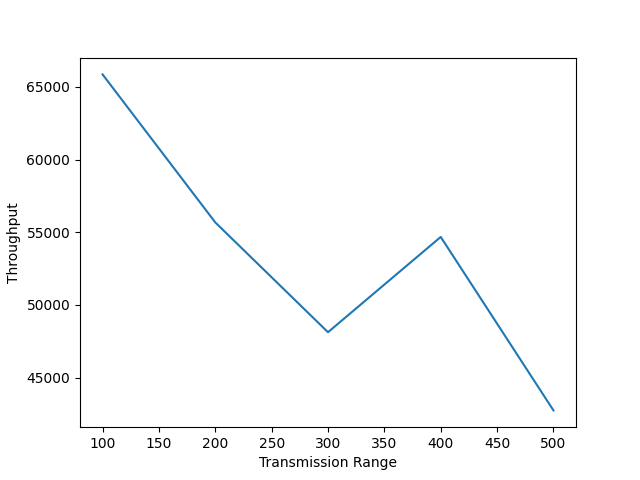
\includegraphics[width=.8\linewidth]{_15_4_static/TransmissionRangevsThroughput.png}
     \caption{Tx Range Vs Throughput}
    \label{tx_range_throughput}    
\end{subfigure}
\begin{subfigure}{.5\textwidth}
  \centering
  % include second image
  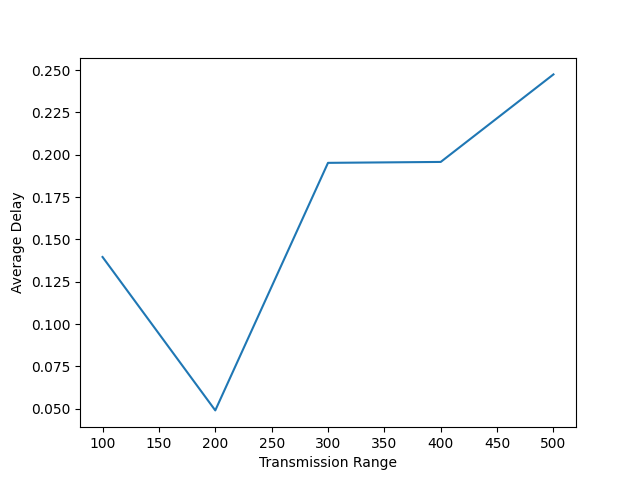
\includegraphics[width=.8\linewidth]{_15_4_static/TransmissionRangevsAverageDelay.png}
    \caption{Tx Range Vs Average Delay}
     \label{tx_range_delay}
\end{subfigure}
\begin{subfigure}{.5\textwidth}
  \centering
  % include third image
  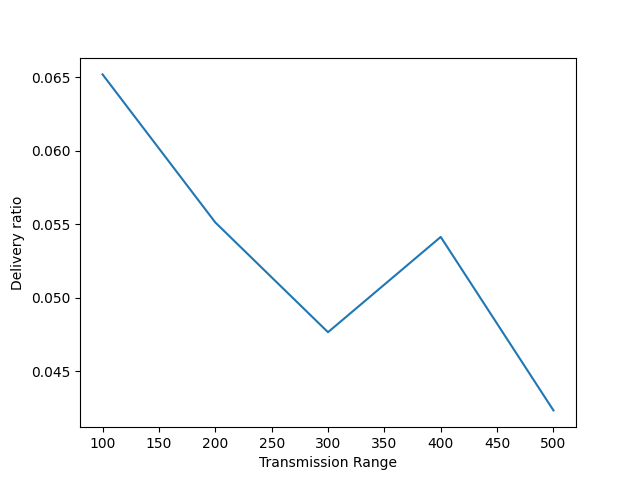
\includegraphics[width=.8\linewidth]{_15_4_static/TransmissionRangevsDeliveryRatio.png}
     \caption{Tx Range Vs Delivary Ratio}
     \label{tx_range_delivery}
\end{subfigure}
\begin{subfigure}{.5\textwidth}
  \centering
  % include fourth image
  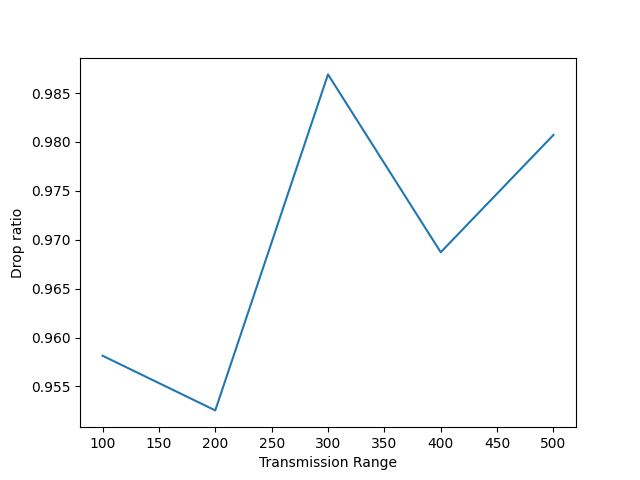
\includegraphics[width=.8\linewidth]{_15_4_static/TransmissionRangevsDropRatio.png}
     \caption{Tx Range Vs Drop Ratio}
     \label{tx_range_drop}
\end{subfigure}
\begin{subfigure}{.5\textwidth}
  \centering
  % include fifth image
  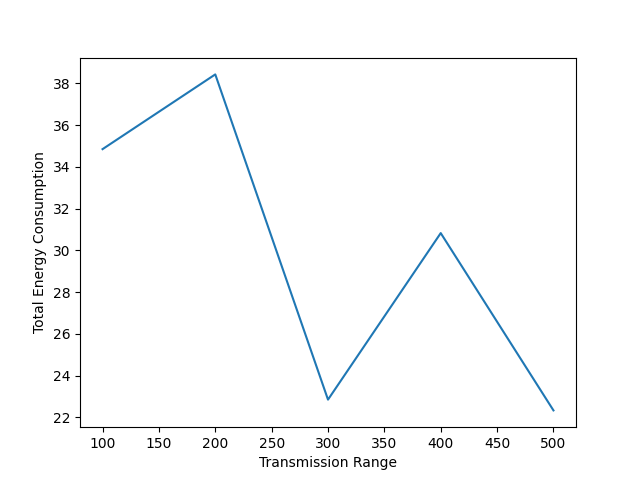
\includegraphics[width=.8\linewidth]{_15_4_static/TransmissionRangevsTotalEnergyConsumption.png}
     \caption{Tx Range Vs Energy Consumption}
     \label{tx_range_energy}
\end{subfigure}
\begin{subfigure}{.5\textwidth}
  \centering
  % include sixth image
  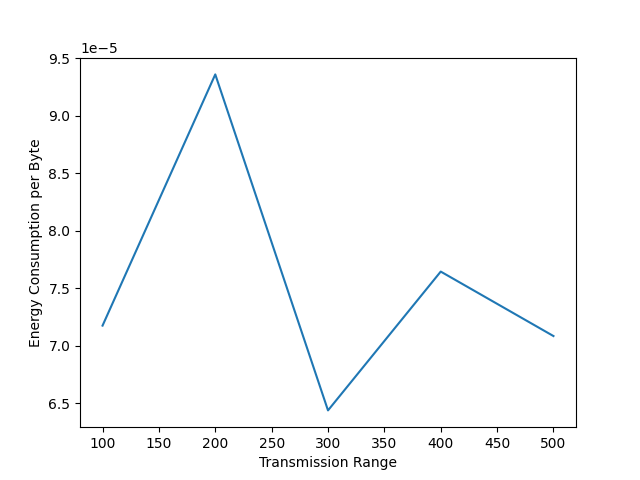
\includegraphics[width=.8\linewidth]{_15_4_static/TransmissionRangevsEnergyConsumptionperByte.png}
     \caption{Tx Range Vs Energy Per Byte}
     \label{tx_range_energy_per_byte}
\end{subfigure}
\caption{Varying Transmission Range}
\label{fig:varyingTxRange}
\end{figure}
\begin{figure}[h]
\begin{subfigure}{.5\textwidth}
  \centering
  % include first image
  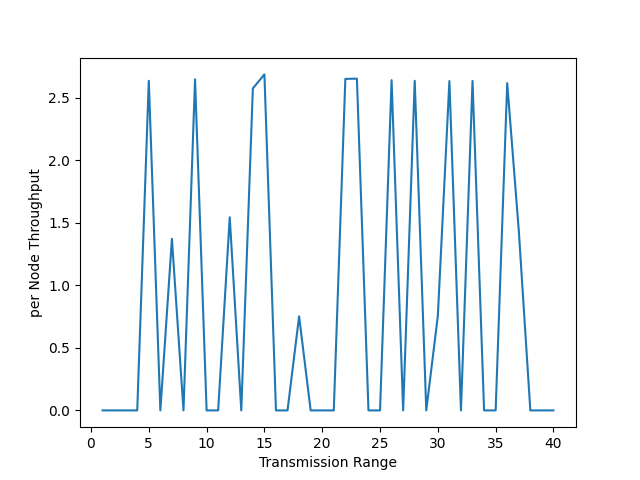
\includegraphics[width=.8\linewidth]{_15_4_static/TransmissionRange(100)vsperNodeThroughput.png}
     \caption{Tx Range(100) Vs Throughput per Node}
 \end{subfigure}
\begin{subfigure}{.5\textwidth}
  \centering
  % include second image
  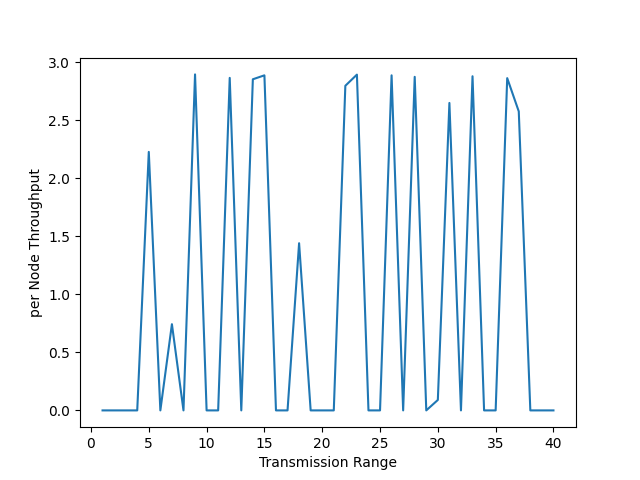
\includegraphics[width=.8\linewidth]{_15_4_static/TransmissionRange(200)vsperNodeThroughput.png}
     \caption{Tx Range(200) Vs Throughput per Node}
    \end{subfigure}
\begin{subfigure}{.5\textwidth}
    \centering
    % include third image
    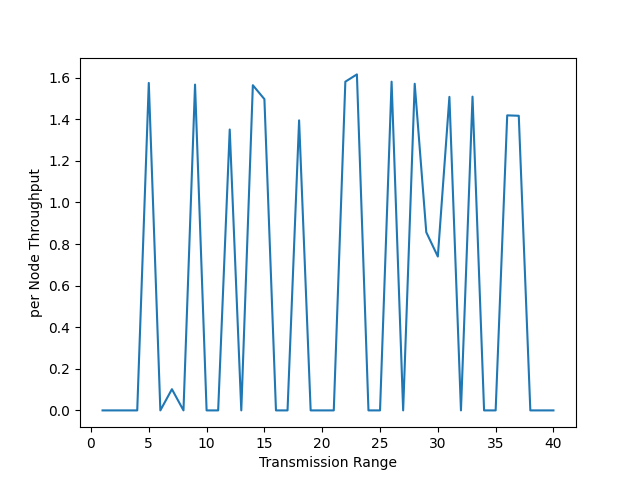
\includegraphics[width=.8\linewidth]{_15_4_static/TransmissionRange(300)vsperNodeThroughput.png}
         \caption{Tx Range(300) Vs Throughput per Node}
        \end{subfigure}
\begin{subfigure}{.5\textwidth}
    \centering
    % include fourth image
    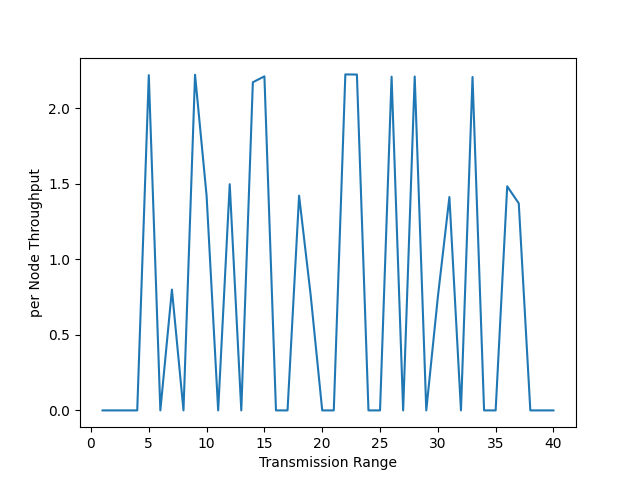
\includegraphics[width=.8\linewidth]{_15_4_static/TransmissionRange(400)vsperNodeThroughput.png}
         \caption{Tx Range(400) Vs Throughput per Node}
        \end{subfigure}
\begin{subfigure}{.5\textwidth}
    \centering
    % include fifth image
    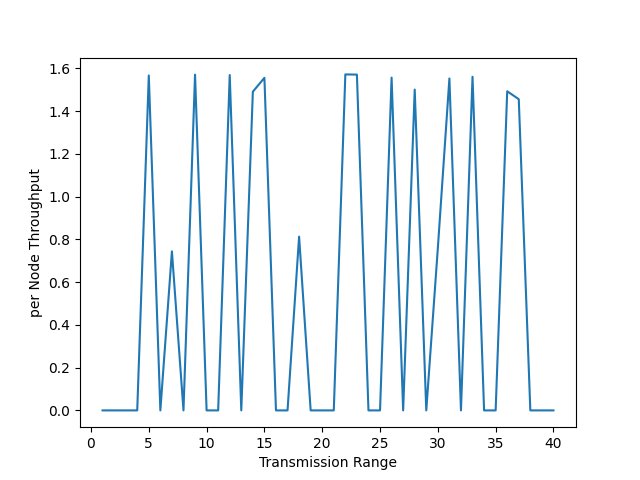
\includegraphics[width=.8\linewidth]{_15_4_static/TransmissionRange(500)vsperNodeThroughput.png}
         \caption{Tx Range(500) Vs Throughput per Node}
        \end{subfigure}
\caption{Varying Transmission Range (Throughput per Node)}
\label{tx_range_per_node_throughput}
\end{figure}



%\section{Wireless IEEE 802.11.2 Mobile Networks}
\subsection{Description of the simulation}
The simulation is based on the IEEE 802.11.2(mobile) standard. Routing is based on the aodv protocol. The simulation is based on the ns-2 simulator. The simulation is based on the following parameters:
\begin{itemize}
    \item Channel: Wireless channel
    \item Propagation: Two-ray ground
    \item Antenna: Omnidirectional
    \item Link: IEEE 802.11.2
    \item Queue: Drop-tail
    \item Routing: AODV
    \item Mobility: Random waypoint
    \item Position: Grid
    \item Area: 500 x 500 meters
    \item Flow: Random source to random destination
    \item Packet size: 64 bytes
    \item Number of nodes: Variable
    \item Number of flows: Variable
    \item Packet rate: Variable
    \item Speed: Variable
    \item Simulation time: 60 seconds
\end{itemize}

\subsection{Results}
\subsubsection{Varying Number of Nodes}
Baseline parameters are as follows:
\begin{itemize}
    \item Number of flows: 20
    \item Packet rate: 100 packets per second
    \item Speed: 5 meters per second
\end{itemize}
The number of nodes is varied from 20 to 100 in steps of 20.
See Figure \ref{node_throughput_mobile} ,\ref{node_delay_mobile} , \ref{node_delivery_mobile} , \ref{node_drop_mobile}, \ref{node_energy_mobile} , \ref{node_energy_mobile_per_byte} and \ref{node_per_node_throughput_mobile} for the result.
\begin{figure}[h]
\begin{subfigure}{.5\textwidth}
  \centering
  % include first image
  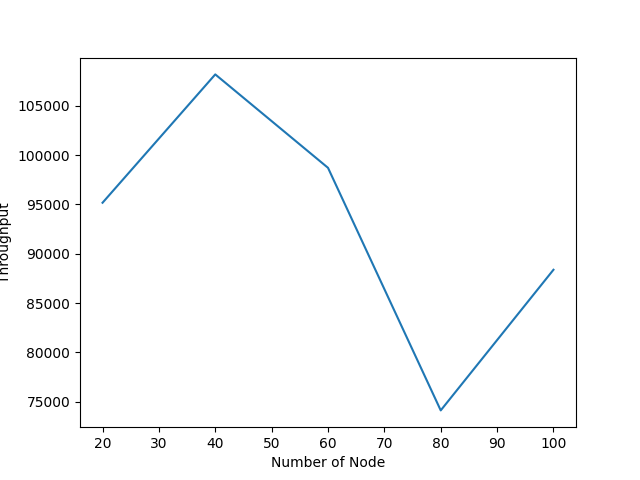
\includegraphics[width=.8\linewidth]{_11_2_mobile/NumberofNodevsThroughput.png}
     \caption{Number of Nodes Vs Throughput}
    \label{node_throughput_mobile}
\end{subfigure}
\begin{subfigure}{.5\textwidth}
  \centering
  % include second image
  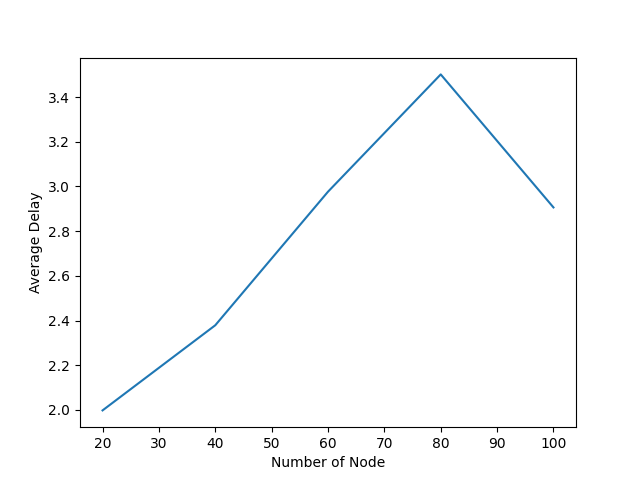
\includegraphics[width=.8\linewidth]{_11_2_mobile/NumberofNodevsAverageDelay.png}
    \caption{Number of Nodes Vs Average Delay}
     \label{node_delay_mobile}
\end{subfigure}
\begin{subfigure}{.5\textwidth}
  \centering
  % include third image
  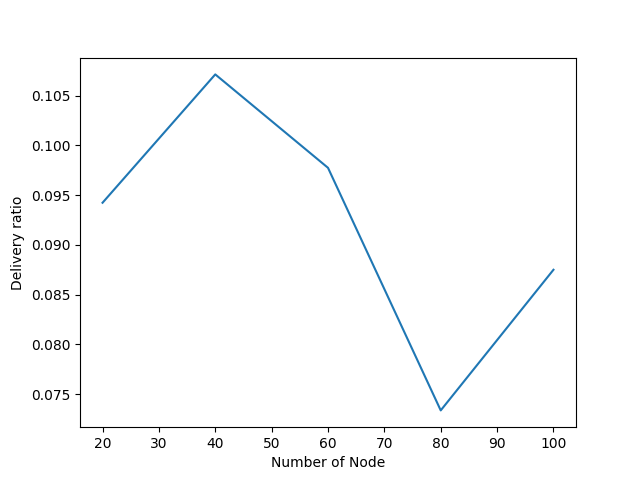
\includegraphics[width=.8\linewidth]{_11_2_mobile/NumberofNodevsDeliveryRatio.png}
     \caption{Number of Nodes Vs Delivary Ratio}
     \label{node_delivery_mobile}
\end{subfigure}
\begin{subfigure}{.5\textwidth}
  \centering
  % include fourth image
  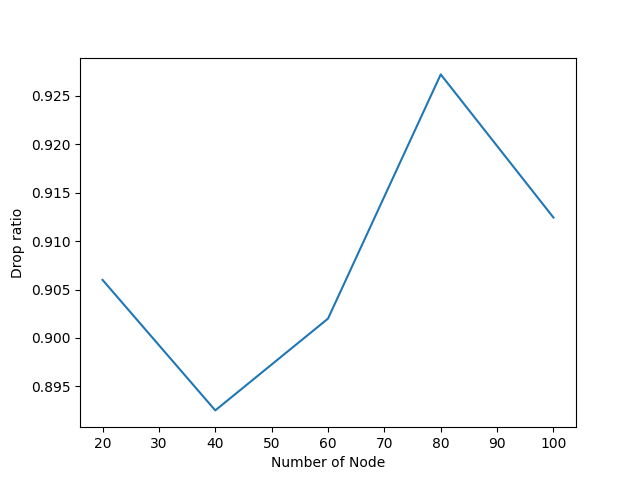
\includegraphics[width=.8\linewidth]{_11_2_mobile/NumberofNodevsDropRatio.png}
     \caption{Number of Nodes Vs Drop Ratio}
     \label{node_drop_mobile}
\end{subfigure}
\begin{subfigure}{.5\textwidth}
  \centering
  % include fifth image
  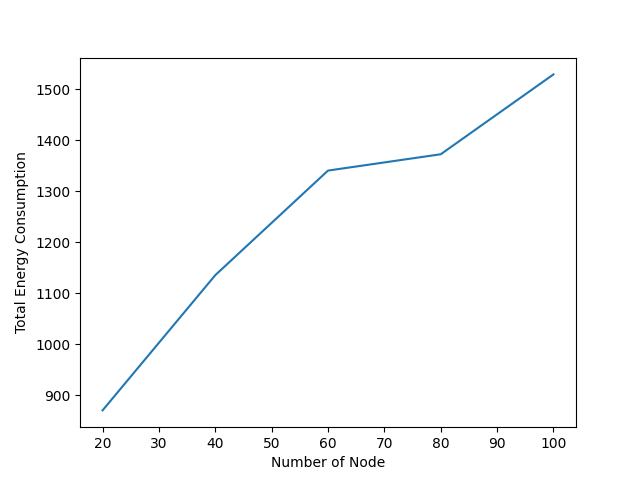
\includegraphics[width=.8\linewidth]{_11_2_mobile/NumberofNodevsTotalEnergyConsumption.png}
     \caption{Number of Nodes Vs Energy Consumption}
     \label{node_energy_mobile}
\end{subfigure}
\begin{subfigure}{.5\textwidth}
  \centering
  % include sixth image
  \includegraphics[width=.8\linewidth]{_11_2_mobile/NumberofNodevsEnergyConsumptionperByte.png}
     \caption{Number of Nodes Vs Energy Per Byte}
     \label{node_energy_mobile_per_byte}
\end{subfigure}
\caption{Varying Number of Nodes}
\label{fig:varyingNode}
\end{figure}
\begin{figure}[h]
\begin{subfigure}{.5\textwidth}
  \centering
  % include first image
  \includegraphics[width=.8\linewidth]{_11_2_mobile/NumberofNode(20)vsperNodeThroughput.png}
     \caption{Number of Nodes(20) Vs Throughput per Node}
 \end{subfigure}
\begin{subfigure}{.5\textwidth}
  \centering
  % include second image
  \includegraphics[width=.8\linewidth]{_11_2_mobile/NumberofNode(40)vsperNodeThroughput.png}
     \caption{Number of Nodes(40) Vs Throughput per Node}
    \end{subfigure}
\begin{subfigure}{.5\textwidth}
    \centering
    % include third image
    \includegraphics[width=.8\linewidth]{_11_2_mobile/NumberofNode(60)vsperNodeThroughput.png}
         \caption{Number of Nodes(60) Vs Throughput per Node}
        \end{subfigure}
\begin{subfigure}{.5\textwidth}
    \centering
    % include fourth image
    \includegraphics[width=.8\linewidth]{_11_2_mobile/NumberofNode(80)vsperNodeThroughput.png}
         \caption{Number of Nodes(80) Vs Throughput per Node}
        \end{subfigure}
\begin{subfigure}{.5\textwidth}
    \centering
    % include fifth image
    \includegraphics[width=.8\linewidth]{_11_2_mobile/NumberofNode(100)vsperNodeThroughput.png}
         \caption{Number of Nodes(100) Vs Throughput per Node}
        \end{subfigure}
\caption{Varying Number of Nodes (Throughput per Node)}
\label{node_per_node_throughput_mobile}
\end{figure}
\subsubsection{Varying Number of Flows}
Baseline parameters are as follows:
\begin{itemize}
    \item Number of nodes: 40
    \item Packet rate: 100 packets per second
    \item Speed: 5 meters per second
\end{itemize}
The number of flows is varied from 10 to 50 in steps of 10.
See Figure \ref{flow_throughput_mobile} ,\ref{flow_delay_mobile} , \ref{flow_delivery_mobile} , \ref{flow_drop_mobile}, \ref{flow_energy_mobile} , \ref{flow_energy_mobile_per_byte} and \ref{flow_per_node_throughput_mobile} for the result.
\begin{figure}[h]
\begin{subfigure}{.5\textwidth}
  \centering
  % include first image
  \includegraphics[width=.8\linewidth]{_11_2_mobile/NumberofFlowvsThroughput.png}
     \caption{Number of Flows Vs Throughput}
    \label{flow_throughput_mobile}
\end{subfigure}
\begin{subfigure}{.5\textwidth}
  \centering
  % include second image
  \includegraphics[width=.8\linewidth]{_11_2_mobile/NumberofFlowvsAverageDelay.png}
    \caption{Number of Flows Vs Average Delay}
     \label{flow_delay_mobile}
\end{subfigure}
\begin{subfigure}{.5\textwidth}
  \centering
  % include third image
  \includegraphics[width=.8\linewidth]{_11_2_mobile/NumberofFlowvsDeliveryRatio.png}
     \caption{Number of Flows Vs Delivary Ratio}
     \label{flow_delivery_mobile}
\end{subfigure}
\begin{subfigure}{.5\textwidth}
  \centering
  % include fourth image
  \includegraphics[width=.8\linewidth]{_11_2_mobile/NumberofFlowvsDropRatio.png}
     \caption{Number of Flows Vs Drop Ratio}
     \label{flow_drop_mobile}
\end{subfigure}
\begin{subfigure}{.5\textwidth}
  \centering
  % include fifth image
  \includegraphics[width=.8\linewidth]{_11_2_mobile/NumberofFlowvsTotalEnergyConsumption.png}
     \caption{Number of Flows Vs Energy Consumption}
     \label{flow_energy_mobile}
\end{subfigure}
\begin{subfigure}{.5\textwidth}
  \centering
  % include sixth image
  \includegraphics[width=.8\linewidth]{_11_2_mobile/NumberofFlowvsEnergyConsumptionperByte.png}
     \caption{Number of Flows Vs Energy Per Byte}
     \label{flow_energy_mobile_per_byte}
\end{subfigure}
\caption{Varying Number of Flows}
\label{fig:varyingFlow}
\end{figure}
\begin{figure}[h]
\begin{subfigure}{.5\textwidth}
  \centering
  % include first image
  \includegraphics[width=.8\linewidth]{_11_2_mobile/NumberofFlow(10)vsperNodeThroughput.png}
     \caption{Number of Flows(10) Vs Throughput per Node}
 \end{subfigure}
\begin{subfigure}{.5\textwidth}
  \centering
  % include second image
  \includegraphics[width=.8\linewidth]{_11_2_mobile/NumberofFlow(20)vsperNodeThroughput.png}
     \caption{Number of Flows(20) Vs Throughput per Node}
    \end{subfigure}
\begin{subfigure}{.5\textwidth}
    \centering
    % include third image
    \includegraphics[width=.8\linewidth]{_11_2_mobile/NumberofFlow(30)vsperNodeThroughput.png}
         \caption{Number of Flows(30) Vs Throughput per Node}
        \end{subfigure}
\begin{subfigure}{.5\textwidth}
    \centering
    % include fourth image
    \includegraphics[width=.8\linewidth]{_11_2_mobile/NumberofFlow(40)vsperNodeThroughput.png}
         \caption{Number of Flows(40) Vs Throughput per Node}
        \end{subfigure}
\begin{subfigure}{.5\textwidth}
    \centering
    % include fifth image
    \includegraphics[width=.8\linewidth]{_11_2_mobile/NumberofFlow(50)vsperNodeThroughput.png}
         \caption{Number of Flows(50) Vs Throughput per Node}
        \end{subfigure}
\caption{Varying Number of Flows (Throughput per Node)}
\label{flow_per_node_throughput_mobile}
\end{figure}

\subsubsection{Varying Packet per Second}
Baseline parameters are as follows:
\begin{itemize}
    \item Number of nodes: 40
    \item Number of flows: 10
    \item Speed: 5 meters per second
\end{itemize}
The packet rate is varied from 100 to 500 packets per second in steps of 100.
See Figure \ref{packet_rate_throughput_mobile} ,\ref{packet_rate_delay_mobile} , \ref{packet_rate_delivery_mobile} , \ref{packet_rate_drop_mobile}, \ref{packet_rate_energy_mobile} , \ref{packet_rate_energy_mobile_per_byte} and \ref{packet_rate_per_node_throughput_mobile} for the result.
\begin{figure}[h]
\begin{subfigure}{.5\textwidth}
  \centering
  % include first image
  \includegraphics[width=.8\linewidth]{_11_2_mobile/PacketpersecondvsThroughput.png}
     \caption{Packet Rate Vs Throughput}
    \label{packet_rate_throughput_mobile}
\end{subfigure}
\begin{subfigure}{.5\textwidth}
  \centering
  % include second image
  \includegraphics[width=.8\linewidth]{_11_2_mobile/PacketpersecondvsAverageDelay.png}
    \caption{Packet Rate Vs Average Delay}
     \label{packet_rate_delay_mobile}
\end{subfigure}
\begin{subfigure}{.5\textwidth}
  \centering
  % include third image
  \includegraphics[width=.8\linewidth]{_11_2_mobile/PacketpersecondvsDeliveryRatio.png}
     \caption{Packet Rate Vs Delivary Ratio}
     \label{packet_rate_delivery_mobile}
\end{subfigure}
\begin{subfigure}{.5\textwidth}
  \centering
  % include fourth image
  \includegraphics[width=.8\linewidth]{_11_2_mobile/PacketpersecondvsDropRatio.png}
     \caption{Packet Rate Vs Drop Ratio}
     \label{packet_rate_drop_mobile}
\end{subfigure}
\begin{subfigure}{.5\textwidth}
  \centering
  % include fifth image
  \includegraphics[width=.8\linewidth]{_11_2_mobile/PacketpersecondvsTotalEnergyConsumption.png}
     \caption{Packet Rate Vs Energy Consumption}
     \label{packet_rate_energy_mobile}
\end{subfigure}
\begin{subfigure}{.5\textwidth}
  \centering
  % include sixth image
  \includegraphics[width=.8\linewidth]{_11_2_mobile/PacketpersecondvsEnergyConsumptionperByte.png}
     \caption{Packet Rate Vs Energy Per Byte}
     \label{packet_rate_energy_mobile_per_byte}
\end{subfigure}
\caption{Varying Packet Rate}
\label{fig:varyingPacketRate}
\end{figure}
\begin{figure}[h]
\begin{subfigure}{.5\textwidth}
  \centering
  % include first image
  \includegraphics[width=.8\linewidth]{_11_2_mobile/Packetpersecond(100)vsperNodeThroughput.png}
     \caption{Packet Rate(100) Vs Throughput per Node}
 \end{subfigure}
\begin{subfigure}{.5\textwidth}
  \centering
  % include second image
  \includegraphics[width=.8\linewidth]{_11_2_mobile/Packetpersecond(200)vsperNodeThroughput.png}
     \caption{Packet Rate(200) Vs Throughput per Node}
    \end{subfigure}
\begin{subfigure}{.5\textwidth}
    \centering
    % include third image
    \includegraphics[width=.8\linewidth]{_11_2_mobile/Packetpersecond(300)vsperNodeThroughput.png}
         \caption{Packet Rate(300) Vs Throughput per Node}
        \end{subfigure}
\begin{subfigure}{.5\textwidth}
    \centering
    % include fourth image
    \includegraphics[width=.8\linewidth]{_11_2_mobile/Packetpersecond(400)vsperNodeThroughput.png}
         \caption{Packet Rate(400) Vs Throughput per Node}
        \end{subfigure}
\begin{subfigure}{.5\textwidth}
    \centering
    % include fifth image
    \includegraphics[width=.8\linewidth]{_11_2_mobile/Packetpersecond(500)vsperNodeThroughput.png}
         \caption{Packet Rate(500) Vs Throughput per Node}
        \end{subfigure}
\caption{Varying Packet Rate (Throughput per Node)}
\label{packet_rate_per_node_throughput_mobile}
\end{figure}

\subsubsection{Varying Speed}
Baseline parameters are as follows:
\begin{itemize}
    \item Number of nodes: 40
    \item Number of flows: 20
    \item Packet Rate: 100 packets per second
\end{itemize}
The speed is varied from 5 to 25 meters per second in steps of 5.
See Figure \ref{speed_throughput_mobile} ,\ref{speed_delay_mobile} , \ref{speed_delivery_mobile} , \ref{speed_drop_mobile}, \ref{speed_energy_mobile} , \ref{speed_energy_mobile_per_byte} and \ref{speed_per_node_throughput_mobile} for the result.
\begin{figure}[h]
\begin{subfigure}{.5\textwidth}
  \centering
  % include first image
  \includegraphics[width=.8\linewidth]{_11_2_mobile/SpeedvsThroughput.png}
     \caption{Speed Vs Throughput}
    \label{speed_throughput_mobile}
\end{subfigure}
\begin{subfigure}{.5\textwidth}
  \centering
  % include second image
  \includegraphics[width=.8\linewidth]{_11_2_mobile/SpeedvsAverageDelay.png}
    \caption{Speed Vs Average Delay}
     \label{speed_delay_mobile}
\end{subfigure}
\begin{subfigure}{.5\textwidth}
  \centering
  % include third image
  \includegraphics[width=.8\linewidth]{_11_2_mobile/SpeedvsDeliveryRatio.png}
     \caption{Speed Vs Delivary Ratio}
     \label{speed_delivery_mobile}
\end{subfigure}
\begin{subfigure}{.5\textwidth}
  \centering
  % include fourth image
  \includegraphics[width=.8\linewidth]{_11_2_mobile/SpeedvsDropRatio.png}
     \caption{Speed Vs Drop Ratio}
     \label{speed_drop_mobile}
\end{subfigure}
\begin{subfigure}{.5\textwidth}
  \centering
  % include fifth image
  \includegraphics[width=.8\linewidth]{_11_2_mobile/SpeedvsTotalEnergyConsumption.png}
     \caption{Speed Vs Energy Consumption}
     \label{speed_energy_mobile}
\end{subfigure}
\begin{subfigure}{.5\textwidth}
  \centering
  % include sixth image
  \includegraphics[width=.8\linewidth]{_11_2_mobile/SpeedvsEnergyConsumptionperByte.png}
     \caption{Speed Vs Energy Per Byte}
     \label{speed_energy_mobile_per_byte}
\end{subfigure}
\caption{Varying Speed}
\label{fig:varyingSpeed}
\end{figure}
\begin{figure}[h]
\begin{subfigure}{.5\textwidth}
  \centering
  % include first image
  \includegraphics[width=.8\linewidth]{_11_2_mobile/Speed(5)vsperNodeThroughput.png}
     \caption{Speed(5) Vs Throughput per Node}
 \end{subfigure}
\begin{subfigure}{.5\textwidth}
  \centering
  % include second image
  \includegraphics[width=.8\linewidth]{_11_2_mobile/Speed(10)vsperNodeThroughput.png}
     \caption{Speed(10) Vs Throughput per Node}
    \end{subfigure}
\begin{subfigure}{.5\textwidth}
    \centering
    % include third image
    \includegraphics[width=.8\linewidth]{_11_2_mobile/Speed(15)vsperNodeThroughput.png}
         \caption{Speed(15) Vs Throughput per Node}
        \end{subfigure}
\begin{subfigure}{.5\textwidth}
    \centering
    % include fourth image
    \includegraphics[width=.8\linewidth]{_11_2_mobile/Speed(20)vsperNodeThroughput.png}
         \caption{Speed(20) Vs Throughput per Node}
        \end{subfigure}
\begin{subfigure}{.5\textwidth}
    \centering
    % include fifth image
    \includegraphics[width=.8\linewidth]{_11_2_mobile/Speed(25)vsperNodeThroughput.png}
         \caption{Speed(25) Vs Throughput per Node}
        \end{subfigure}
\caption{Varying Speed (Throughput per Node)}
\label{speed_per_node_throughput_mobile}
\end{figure}



\section{Modified AODV Routing Protocol}
\subsection{Proposed Algorithm}
The below Algorithm is proposed by The paper:


A new field will be added in
the RREQ for calculating transmission energy. The format of
the new RREQ will be


<source\_address, dest\_sequence\_id, source\_sequence\_id,
broadcast\_id, dest\_address, hop\_count, transmission\_energy>
Now based on each packets Transmission energy:
\begin{algorithmic}
\State Calculate drop factor d for every transmitting node.
\State Generate a random number between $0 and 1.$
\If {$random\_value > drop factor$}
    \State broadcast/forward RREQ\_packet,
\Else
\State drop RREQ\_packet.
\EndIf
\end{algorithmic}
This algorithm has some major problem. It always drop packet when network isn't congested at all.
I propose a modification on this algorithm. The idea is to count last $d$ seconds RREQ packet number and drop packet if number of packet cross the average.

\begin{algorithmic}
\State $average \gets get\_average\_per\_second()$
\State $number\_of\_packet\_in\_last\_second \gets get\_last\_second\_count()$
\State Calculate drop factor d for every transmitting node.
\State Generate a random number between 0 and 1.
\If {$number\_of\_packet\_in\_last\_second < average \And random\_value > drop factor$}
    \State broadcast/forward RREQ\_packet,
\Else
\State drop RREQ\_packet.
\EndIf
\end{algorithmic}

\subsection{Implementation}
The following code is added to aodv.cc in AODV::recvRequest(Packet *p) function:
\begin{lstlisting}[language=c]
int flag = 0;
 while(current_time< (int)CURRENT_TIME){
    current_time++;
    for(int i=0;i<MAX_SECOND-1;i++){
      rreq_count[i]  = rreq_count[i+1] ;
    }
    rreq_count[MAX_SECOND-1] = 0;
 }
  rreq_count[MAX_SECOND-1]++;
 // calculating average rreq count
  int sum = 0;
  for(int i=0;i<MAX_SECOND;i++){
    sum += rreq_count[i];
  }
  double avg = (double)sum/MAX_SECOND;
  // drop if high rreq count
  if(avg<rreq_count[MAX_SECOND-1]){
    flag = 1;
  }
// drop if low energy
double drop_prob = 1.0 - 
    (double)rq->rq_transmission_energy/AODV_MAX_TRANSMISSION_ENERGY;
// decrease Transmission Energy
if(rq->rq_transmission_energy>1){
  rq->rq_transmission_energy--;
}

/* -------- more code ----*/
/*
  * Can't reply. So forward the  Route Request
  */
 else {
 	if((Random::uniform() < drop_prob) && flag==1){
  	Packet::free(p);
  	fprintf(stderr,"freeing packet\n");
  	return;
	}
   ih->saddr() = index;
   ih->daddr() = IP_BROADCAST;
   rq->rq_hop_count += 1;
   // Maximum sequence number seen en route
   if (rt) rq->rq_dst_seqno = max(rt->rt_seqno, rq->rq_dst_seqno);
   forward((aodv_rt_entry*) 0, p, DELAY);
 }
\end{lstlisting}
While sending a packet initially, I set the energy to a certain value.
Code in AODV::sendRequest(nsaddr\_t dst)
\begin{lstlisting}
 // Fill up some more fields. 
 rq->rq_type = AODVTYPE_RREQ;
 rq->rq_hop_count = 1;
 rq->rq_bcast_id = bid++;
 rq->rq_dst = dst;
 rq->rq_dst_seqno = (rt ? rt->rt_seqno : 0);
 rq->rq_src = index;
 seqno += 2;
 rq->rq_transmission_energy= AODV_MAX_TRANSMISSION_ENERGY;
 assert ((seqno%2) == 0);
 rq->rq_src_seqno = seqno;
 rq->rq_timestamp = CURRENT_TIME;
\end{lstlisting}
And the new packet Type -> Code snipped from packet.h
\begin{lstlisting}
struct hdr_aodv_request {
    u_int8_t        rq_type;	// Packet Type
    u_int8_t        reserved[2];
    u_int8_t        rq_hop_count;   // Hop Count
    u_int32_t       rq_bcast_id;    // Broadcast ID

    nsaddr_t        rq_dst;         // Destination IP Address
    u_int32_t       rq_dst_seqno;   // Destination Sequence Number
    nsaddr_t        rq_src;         // Source IP Address
    u_int32_t       rq_src_seqno;   // Source Sequence Number
        
    u_int8_t        rq_transmission_energy; // Transmission Energy

    double          rq_timestamp;   // when REQUEST sent;
}
\end{lstlisting}
\subsection{Results}
\subsubsection{Description of the simulation}
The simulation is based on the IEEE 802.11.2(mobile) standard. Routing is based on the aodv protocol. The simulation is based on the ns-2 simulator. The simulation is based on the following parameters:
\begin{itemize}
    \item Channel: Wireless channel
    \item Propagation: Two-ray ground
    \item Antenna: Omnidirectional
    \item Link: IEEE 802.11.2
    \item Queue: Drop-tail
    \item Routing: AODV
    \item Mobility: Random waypoint
    \item Position: Grid
    \item Area: 1000 x 1000 meters
    \item Flow: Random source to random destination
    \item Packet size: 64 bytes
    \item Number of nodes: Variable
    \item Number of flows: Variable
    \item Packet rate: Variable
    \item Speed: Variable
    \item Simulation time: 60 seconds
\end{itemize}
\subsubsection{Results}
Varying Number of Node.
Baseline parameters are as follows:
\begin{itemize}
    \item Number of flows: 20
    \item Packet rate: 100 packets per second
    \item Speed: 5 meters per second
\end{itemize}
The number of nodes is varied from 20 to 100 in steps of 20.
See Figure \ref{node_throughput_modified} ,\ref{node_delay_modified} , \ref{node_delivery_modified} , \ref{node_drop_modified}, \ref{node_energy_modified} and \ref{node_energy_modified_per_byte}  for the result.
\begin{figure}[h]
\begin{subfigure}{.5\textwidth}
  \centering
  % include first image
  \includegraphics[width=.8\linewidth]{modified_fig/NumberofNodevsThroughput.png}
     \caption{Number of Nodes Vs Throughput}
    \label{node_throughput_modified}
\end{subfigure}
\begin{subfigure}{.5\textwidth}
  \centering
  % include second image
  \includegraphics[width=.8\linewidth]{modified_fig/NumberofNodevsAverageDelay.png}
    \caption{Number of Nodes Vs Average Delay}
     \label{node_delay_modified}
\end{subfigure}
\begin{subfigure}{.5\textwidth}
  \centering
  % include third image
  \includegraphics[width=.8\linewidth]{modified_fig/NumberofNodevsDeliveryRatio.png}
     \caption{Number of Nodes Vs Delivary Ratio}
     \label{node_delivery_modified}
\end{subfigure}
\begin{subfigure}{.5\textwidth}
  \centering
  % include fourth image
  \includegraphics[width=.8\linewidth]{modified_fig/NumberofNodevsDropRatio.png}
     \caption{Number of Nodes Vs Drop Ratio}
     \label{node_drop_modified}
\end{subfigure}
\begin{subfigure}{.5\textwidth}
  \centering
  % include fifth image
  \includegraphics[width=.8\linewidth]{modified_fig/NumberofNodevsTotalEnergyConsumption.png}
     \caption{Number of Nodes Vs Energy Consumption}
     \label{node_energy_modified}
\end{subfigure}
\begin{subfigure}{.5\textwidth}
  \centering
  % include sixth image
  \includegraphics[width=.8\linewidth]{modified_fig/NumberofNodevsEnergyConsumptionperByte.png}
     \caption{Number of Nodes Vs Energy Per Byte}
     \label{node_energy_modified_per_byte}
\end{subfigure}
\caption{Varying Number of Nodes}
\label{fig:varyingNode}
\end{figure}

Varying Number of Flows.
Baseline parameters are as follows:
\begin{itemize}
    \item Number of nodes: 60
    \item Packet rate: 100 packets per second
    \item Speed: 5 meters per second
\end{itemize}
The number of flows is varied from 10 to 50 in steps of 10.
See Figure \ref{flow_throughput_modified} ,\ref{flow_delay_modified} , \ref{flow_delivery_modified} , \ref{flow_drop_modified}, \ref{flow_energy_modified} and \ref{flow_energy_modified_per_byte} for the result.
\begin{figure}[h]
\begin{subfigure}{.5\textwidth}
  \centering
  % include first image
  \includegraphics[width=.8\linewidth]{modified_fig/NumberofFlowvsThroughput.png}
     \caption{Number of Flows Vs Throughput}
    \label{flow_throughput_modified}
\end{subfigure}
\begin{subfigure}{.5\textwidth}
  \centering
  % include second image
  \includegraphics[width=.8\linewidth]{modified_fig/NumberofFlowvsAverageDelay.png}
    \caption{Number of Flows Vs Average Delay}
     \label{flow_delay_modified}
\end{subfigure}
\begin{subfigure}{.5\textwidth}
  \centering
  % include third image
  \includegraphics[width=.8\linewidth]{modified_fig/NumberofFlowvsDeliveryRatio.png}
     \caption{Number of Flows Vs Delivary Ratio}
     \label{flow_delivery_modified}
\end{subfigure}
\begin{subfigure}{.5\textwidth}
  \centering
  % include fourth image
  \includegraphics[width=.8\linewidth]{modified_fig/NumberofFlowvsDropRatio.png}
     \caption{Number of Flows Vs Drop Ratio}
     \label{flow_drop_modified}
\end{subfigure}
\begin{subfigure}{.5\textwidth}
  \centering
  % include fifth image
  \includegraphics[width=.8\linewidth]{modified_fig/NumberofFlowvsTotalEnergyConsumption.png}
     \caption{Number of Flows Vs Energy Consumption}
     \label{flow_energy_modified}
\end{subfigure}
\begin{subfigure}{.5\textwidth}
  \centering
  % include sixth image
  \includegraphics[width=.8\linewidth]{modified_fig/NumberofFlowvsEnergyConsumptionperByte.png}
     \caption{Number of Flows Vs Energy Per Byte}
     \label{flow_energy_modified_per_byte}
\end{subfigure}
\caption{Varying Number of Flows}
\label{fig:varyingFlow}
\end{figure}


Varying Packet per Second.Baseline parameters are as follows:
\begin{itemize}
    \item Number of nodes: 60
    \item Number of flows: 10
    \item Speed: 5 meters per second
\end{itemize}
The packet rate is varied from 100 to 500 packets per second in steps of 100.
See Figure \ref{packet_rate_throughput_modified} ,\ref{packet_rate_delay_modified} , \ref{packet_rate_delivery_modified} , \ref{packet_rate_drop_modified}, \ref{packet_rate_energy_modified} and \ref{packet_rate_energy_modified_per_byte}  for the result.
\begin{figure}[h]
\begin{subfigure}{.5\textwidth}
  \centering
  % include first image
  \includegraphics[width=.8\linewidth]{modified_fig/PacketpersecondvsThroughput.png}
     \caption{Packet Rate Vs Throughput}
    \label{packet_rate_throughput_modified}
\end{subfigure}
\begin{subfigure}{.5\textwidth}
  \centering
  % include second image
  \includegraphics[width=.8\linewidth]{modified_fig/PacketpersecondvsAverageDelay.png}
    \caption{Packet Rate Vs Average Delay}
     \label{packet_rate_delay_modified}
\end{subfigure}
\begin{subfigure}{.5\textwidth}
  \centering
  % include third image
  \includegraphics[width=.8\linewidth]{modified_fig/PacketpersecondvsDeliveryRatio.png}
     \caption{Packet Rate Vs Delivary Ratio}
     \label{packet_rate_delivery_modified}
\end{subfigure}
\begin{subfigure}{.5\textwidth}
  \centering
  % include fourth image
  \includegraphics[width=.8\linewidth]{modified_fig/PacketpersecondvsDropRatio.png}
     \caption{Packet Rate Vs Drop Ratio}
     \label{packet_rate_drop_modified}
\end{subfigure}
\begin{subfigure}{.5\textwidth}
  \centering
  % include fifth image
  \includegraphics[width=.8\linewidth]{modified_fig/PacketpersecondvsTotalEnergyConsumption.png}
     \caption{Packet Rate Vs Energy Consumption}
     \label{packet_rate_energy_modified}
\end{subfigure}
\begin{subfigure}{.5\textwidth}
  \centering
  % include sixth image
  \includegraphics[width=.8\linewidth]{modified_fig/PacketpersecondvsEnergyConsumptionperByte.png}
     \caption{Packet Rate Vs Energy Per Byte}
     \label{packet_rate_energy_modified_per_byte}
\end{subfigure}
\caption{Varying Packet Rate}
\label{fig:varyingPacketRate}
\end{figure}

Varying Speed.
Baseline parameters are as follows:
\begin{itemize}
    \item Number of nodes: 60
    \item Number of flows: 20
    \item Packet Rate: 100 packets per second
\end{itemize}
The speed is varied from 5 to 25 meters per second in steps of 5.
See Figure \ref{speed_throughput_modified} ,\ref{speed_delay_modified} , \ref{speed_delivery_modified} , \ref{speed_drop_modified}, \ref{speed_energy_modified} and \ref{speed_energy_modified_per_byte}  for the result.
\begin{figure}[h]
\begin{subfigure}{.5\textwidth}
  \centering
  % include first image
  \includegraphics[width=.8\linewidth]{modified_fig/SpeedvsThroughput.png}
     \caption{Speed Vs Throughput}
    \label{speed_throughput_modified}
\end{subfigure}
\begin{subfigure}{.5\textwidth}
  \centering
  % include second image
  \includegraphics[width=.8\linewidth]{modified_fig/SpeedvsAverageDelay.png}
    \caption{Speed Vs Average Delay}
     \label{speed_delay_modified}
\end{subfigure}
\begin{subfigure}{.5\textwidth}
  \centering
  % include third image
  \includegraphics[width=.8\linewidth]{modified_fig/SpeedvsDeliveryRatio.png}
     \caption{Speed Vs Delivary Ratio}
     \label{speed_delivery_modified}
\end{subfigure}
\begin{subfigure}{.5\textwidth}
  \centering
  % include fourth image
  \includegraphics[width=.8\linewidth]{modified_fig/SpeedvsDropRatio.png}
     \caption{Speed Vs Drop Ratio}
     \label{speed_drop_modified}
\end{subfigure}
\begin{subfigure}{.5\textwidth}
  \centering
  % include fifth image
  \includegraphics[width=.8\linewidth]{modified_fig/SpeedvsTotalEnergyConsumption.png}
     \caption{Speed Vs Energy Consumption}
     \label{speed_energy_modified}
\end{subfigure}
\begin{subfigure}{.5\textwidth}
  \centering
  % include sixth image
  \includegraphics[width=.8\linewidth]{modified_fig/SpeedvsEnergyConsumptionperByte.png}
     \caption{Speed Vs Energy Per Byte}
     \label{speed_energy_modified_per_byte}
\end{subfigure}
\caption{Varying Speed}
\label{fig:varyingSpeed}
\end{figure}

\subsection{Findings}
Almost in every simulation, modified algorithm did better performance than the existing algorithm.In throughput, Delivery Ratio as well as in every parameters, modified algorithm did perform better.Findings are:
\begin{itemize}
  \item Existing AODV Does't perform well in big topology and where large number of communication is going on.
  \item A proverb goes -"The game
is not worth the candle." Meaning is- Number of RREQ packet is increased so much that it congested the overall network. So it should be handle carefully.
  \item My solution works well as it tries to minimize redundant RREQ Packet by droping them when they tries to congest the network
  \item RREQ packet shouldn't send blindly. It should manage more intelligently like a node can use previous experience to selectively send packet to those node which resolve RREQ request recently.Those node will be more tented to connected with other node. 
  \item This approach is also energy efficient. As it forward less packet than the existing protocol, It saves energy.And Energy is important in network like this where there is no infrastructure.
\end{itemize}
% \section{Discussion}
% \subsection{Varying Number of Node}
% This data shows the results of a simulation of a wireless network with a fixed area of 500 and 20 flows, but varying number of nodes, from 20 to 100.

% As the number of nodes in the network increases, the drop ratio also increases, indicating that the network becomes more congested and there is a higher likelihood of packets being dropped(See \ref{fig:varyingNode}). The average delay also increases with the number of nodes, reflecting the increased competition for resources in the network. On the other hand, the throughput and delivery ratio both decrease, which suggests that the network becomes less efficient as the number of nodes increases.
% \subsection{Varying Number of flow}
% This data provides information about the performance of a wireless communication network in a 500 square area with 40 nodes. The number of flows (number of data streams transmitted in parallel) varies from 10 to 50.

% The results show that the number of dropped packets increases as the number of flows increases. When the number of flows is 10, the drop ratio is 47.99\% and the delivery ratio is 51.34\%. As the number of flows increases, the drop ratio increases and the delivery ratio decreases. When the number of flows is 50, the drop ratio is 96.27\% and the delivery ratio is only 2.79\%(\ref{fig:varyingFlow}).

% Additionally, the average delay and throughput of the network decrease as the number of flows increases. When the number of flows is 10, the average delay is 1.534 seconds and the throughput is 459553 bits/sec. When the number of flows is 50, the average delay is 7.608 seconds and the throughput is 130277 bits/sec.
% \subsection{Varying Area}
% This data set represents the results of a simulation experiment that studies the impact of the area on network performance. The network has 40 nodes and 20 flows, and the area of the network is varied from 250 to 1250. The key performance metrics considered are throughput, average delay, delivery ratio, and drop ratio.

% The results show that as the area of the network increases, the average delay and drop ratio increase, while the throughput and delivery ratio decrease(See \ref{fig:varyingArea}). This can be attributed to the fact that with an increase in the area of the network, the number of hops for a packet to reach its destination increases, which results in increased delay and drop ratio. Furthermore, with an increase in the area, the number of nodes in the network also increases, which results in increased competition for network resources and decreased throughput and delivery ratio.

% The data also suggests that the network performance is not uniform for all areas and that there are trade-offs between different performance metrics. For example, in the case of an area of 1250, the network has a higher throughput and delivery ratio compared to other areas, but the average delay is also high. Hence, it is important to consider the specific requirements of a network and make informed decisions while choosing the appropriate network area.

\end{document}
